\documentclass{article}
\usepackage[utf8]{inputenc}
\usepackage{geometry}
\geometry{letterpaper}                   	
\usepackage{graphicx}	
\graphicspath{{images/}}			
\usepackage{float}							
\usepackage{listings}								 	
\usepackage{amssymb}
\usepackage[T1]{fontenc}
\usepackage[framed,numbered,autolinebreaks,useliterate]{mcode}
\title{MAT 128B Project 1}
\author{Xinke Yu, Xuanchen Yu}
\date{February 2018}

\begin{document}

\maketitle
\textbf{Link to Github: https://github.com/xinkeyu/MAT128B}
\section{An Introduction to Fractals}
The \textbf{orbit}  of $z_0$ under $\phi$ is the sequence generated by repeated application of the mapping $\phi (z)$ with initial value $z_0$.\\
The \textbf{filled Julia set} of a polynomial function $\phi(z)$ is the set of points $z_0$ for which the orbit remains bounded.\\
The \textbf{Julia set} is the boundary of a filled Julia set.\\
The \textbf{Mandelbrot set} is the set of points $c$ such that $\phi(z) = z^2 + c$ does not diverge when starting with $z_0 = 0$.\\
\begin{figure}[!hbp]
  \centering
  \begin{minipage}[b]{0.45\textwidth}
    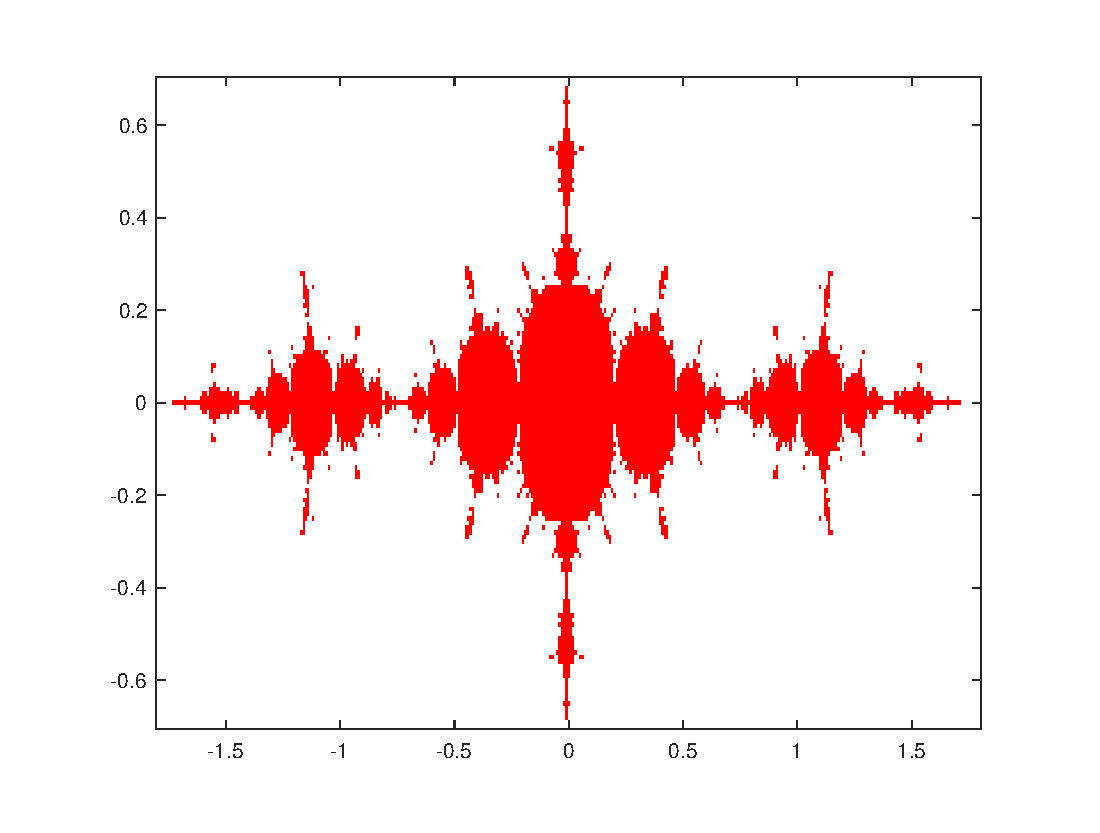
\includegraphics[width=\textwidth]{JuliaSet_fig413.eps}
    \caption{$\phi(z)=z^2-1.25$}
  \end{minipage}
  \hfill
  \begin{minipage}[b]{0.45\textwidth}
    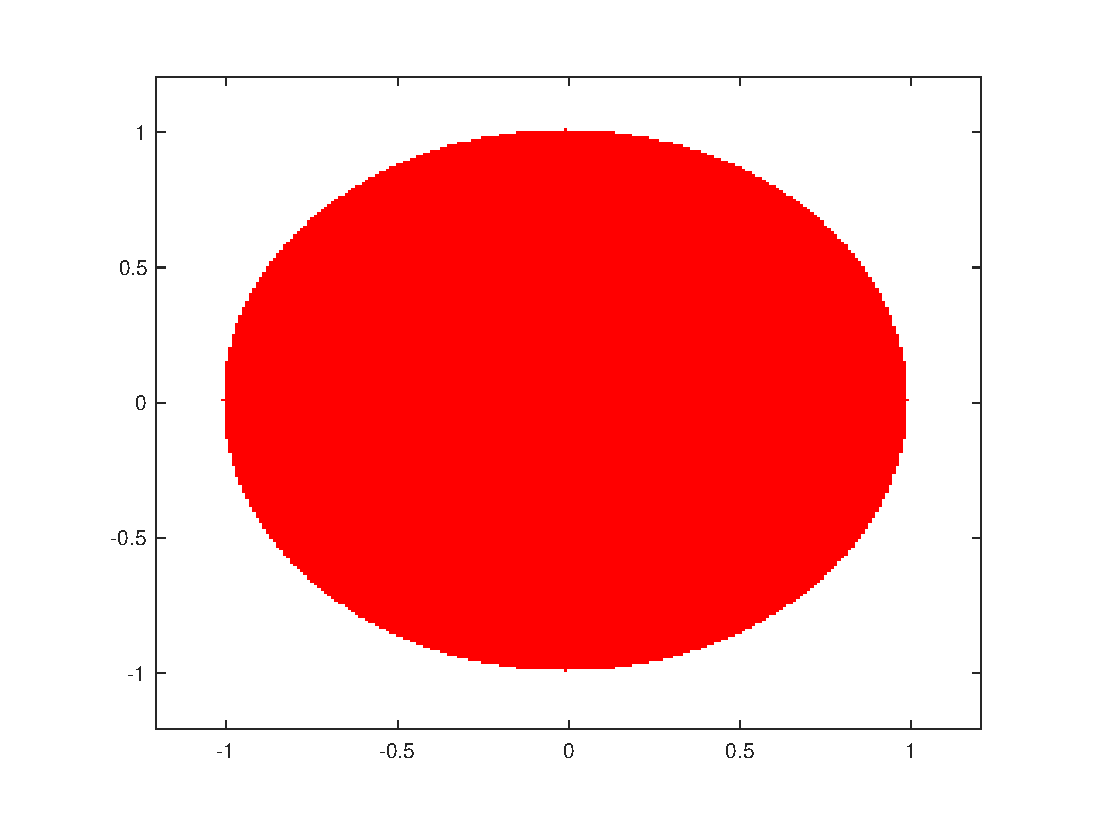
\includegraphics[width=\textwidth]{juliaSet_z2.eps}
    \caption{$\phi(z)=z^2$}
  \end{minipage}
\end{figure}


\section{Generate other examples changing the value of c}
When $z_0$ changes, $\phi(z)$ will either converge or diverge depending on the value of c. However, for any $c$ value, the iteration method diverges when $|z|> 2$. (Hence in the program $z_0$ are chosen within $[-2,2]\times[-2,2]$).\\
The filled Julia sets for different values of c:\\
\begin{figure}[H]
  \centering
  \begin{minipage}[b]{0.45\textwidth}
    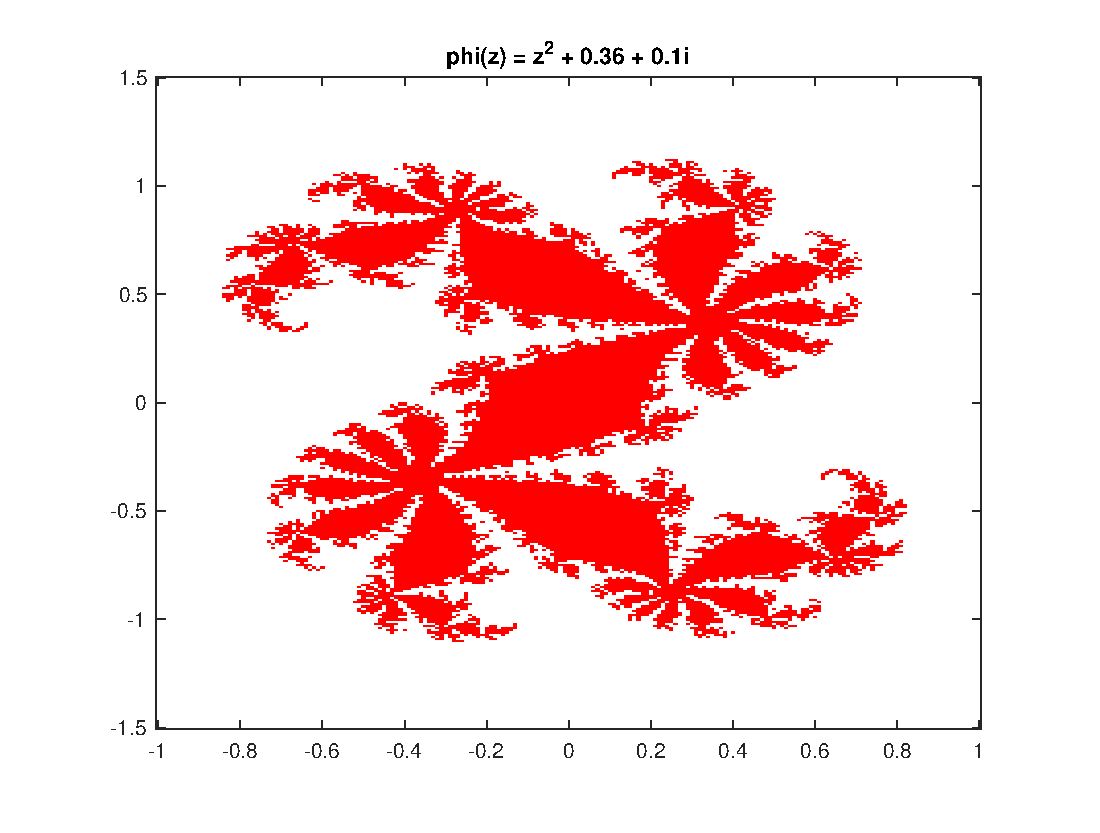
\includegraphics[width=\textwidth]{part2func1.eps}
    \caption{$c = 0.36 + 0.1i$}
  \end{minipage}
  \hfill
  \begin{minipage}[b]{0.45\textwidth}
    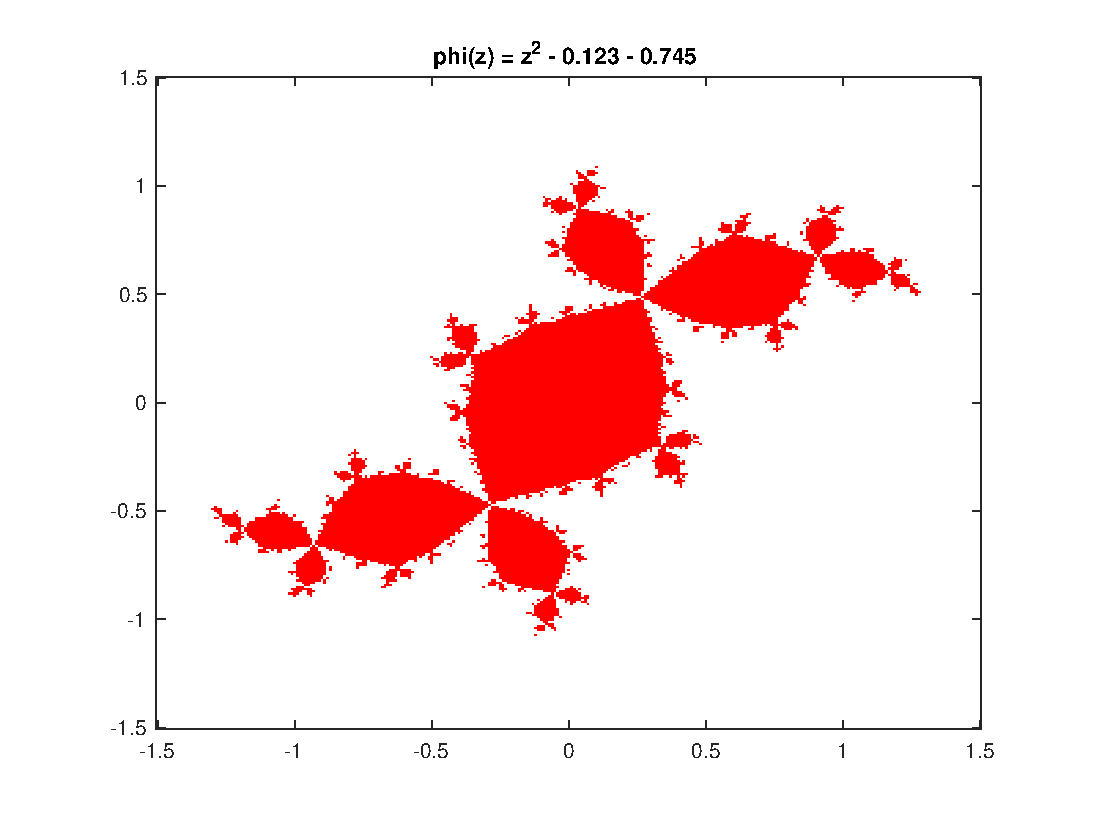
\includegraphics[width=\textwidth]{part2func2.eps}
    \caption{$c = -0.123 - 0.745i$}
  \end{minipage}
   \end{figure}
   
   \begin{figure}[!h]
  \begin{minipage}[b]{0.45\textwidth}
    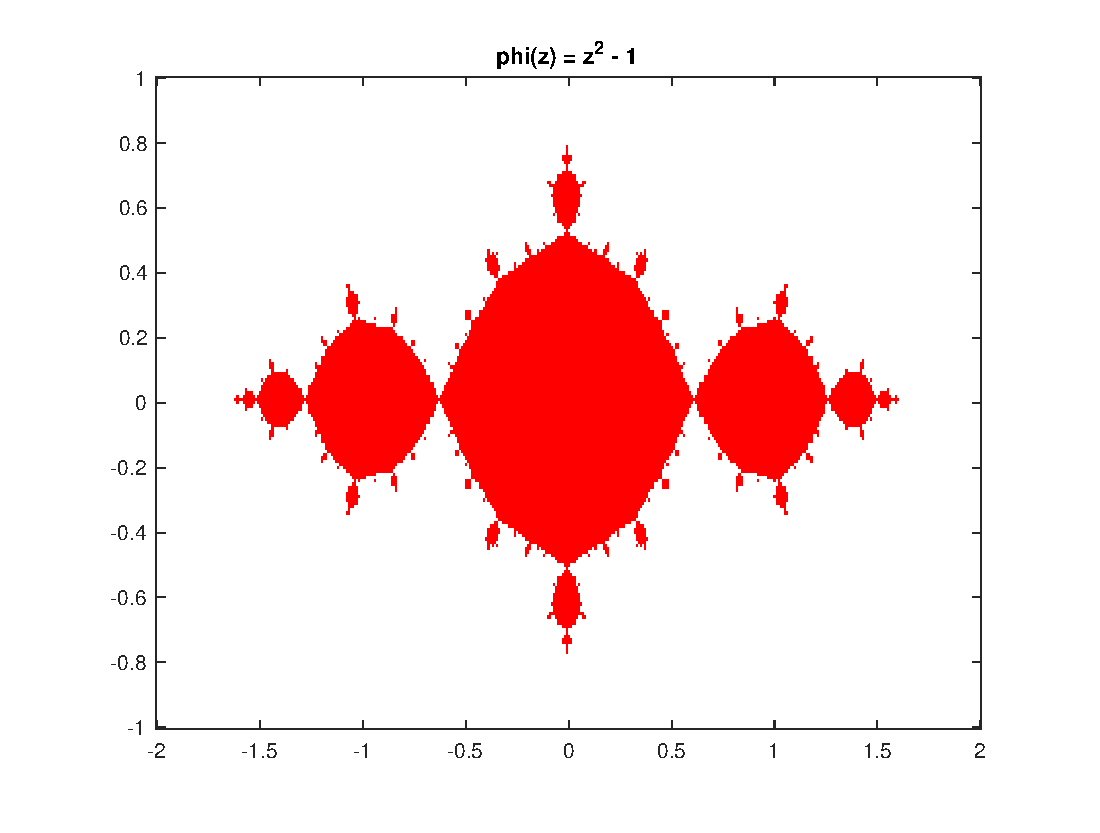
\includegraphics[width=\textwidth]{part2func5.eps}
    \caption{$c = -1$}
  \end{minipage}
  \hfill
  \begin{minipage}[b]{0.45\textwidth}
    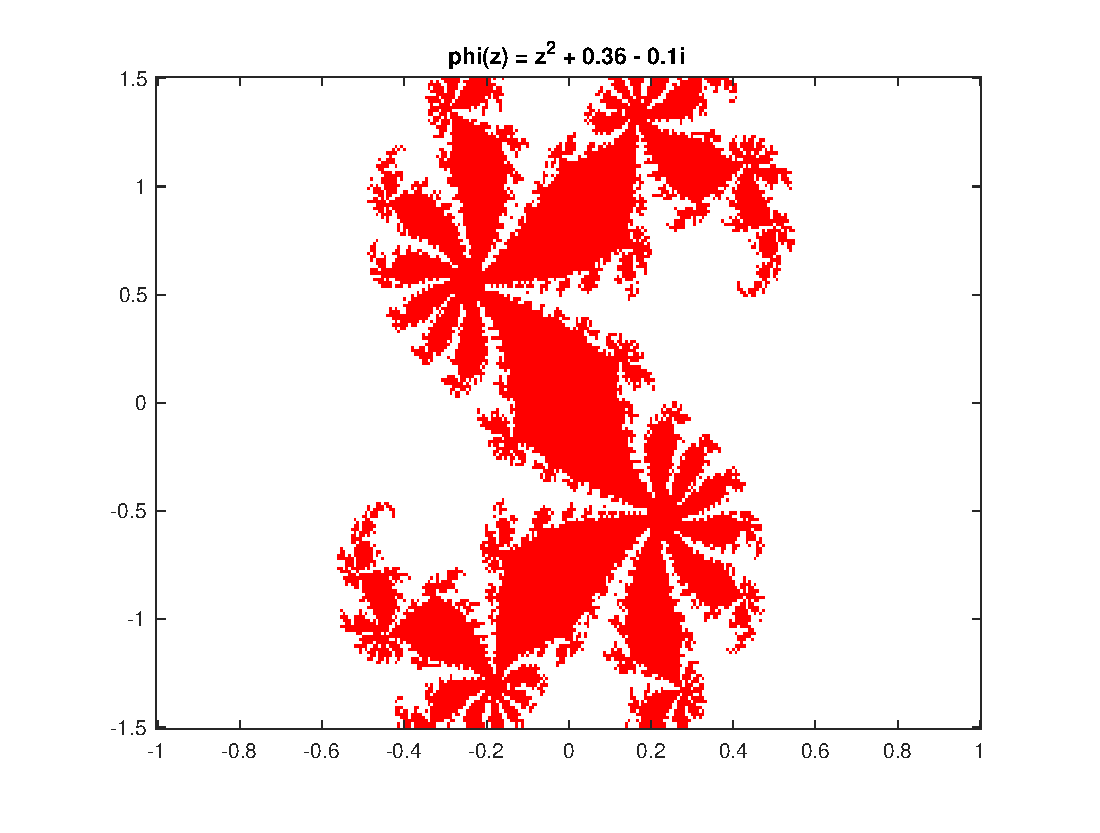
\includegraphics[width=\textwidth]{part2func6.eps}
    \caption{$c = 0.36 - 0.1i$}
  \end{minipage}

\end{figure}

\section{Constructing the Julia Set}
$$z_{n+1} = z_n^2 +c\rightarrow \textrm{ the inverse is: }z_{n+1} = \pm\sqrt{z_{n}-c}$$\\
Let $z_{n+1} = x_{n+1} + iy_{n+1}, z_n = x_n + iy_n$, and $c = x_0 + iy_0$.\\
Then $$x_{n+1}+iy_{n+1} = \pm\sqrt{x_n+iy_n-x_0-iy_0} = \pm\sqrt{(x_n-x_0)-i(y_n-y_0)} $$
Let $(x_n-x_0)-i(y_n-y_0) = re^{i\theta}$.\\
Then $$x_{n+1}+iy_{n+1} =\pm \sqrt{r}e^{i\frac{\theta}{2}} = \pm\sqrt{r}(\cos(\frac{\theta}{2})+i\sin(\frac{\theta}{2}))$$,\\
where $$r = \sqrt{(x_n-x_0)^2 + (y_n-y_0)^2},$$$$ \theta = \tan^{-1}{\frac{y_n-y_0}{x_n-x_0}}\textrm{  (add $\pi$ to $\theta$ if $x_n-x_0 < 0$)}$$
Therefore, $$x_{n+1} = \pm\sqrt{r}\cos(\frac{\theta}{2}) \textrm{, }y_{n+1} = \pm\sqrt{r}\sin(\frac{\theta}{2})$$
Keep applying these two iterations ($x_n$ generates the real part and $y_n$ generates the imaginary part) while randomly choosing the branches for the square root will generate the Julia set.\\
\\
\textbf{Matlab Code}:
\begin{lstlisting}
function [] = constructJuliaSet(x,y)
%construct the Julia set for c = x+iy
numofIt = 200; %number of iterations
rangeUpper = 541; %determines the number of z_n's
increment = 4/(rangeUpper-1);
c = x+1i*y;

plotvecx = zeros(1,rangeUpper^2);%vectors that store the points
plotvecy = zeros(1,rangeUpper^2);

index = 1;
for i = 1: rangeUpper %choose initial values from -2 to 2
    x_co = -2 + (rangeUpper-1)*increment;%real part
    for j = 1: rangeUpper 
       y_co = -2 + (rangeUpper-1)*increment;%imaginary part 
       rnew = sqrt(sqrt((x_co-x)^2+(y_co-y)^2));
       theta = atan((y_co-y)/(x_co-x));
       if(x_co-x)<0
           theta = theta + pi;
       end
       xnew = rnew * cos(theta/2);
       ynew = rnew * sin(theta/2);
       k = 0;

       while k <= numofIt
           k = k + 1;
           randNum = round(rand()); %random number that determines which branch to pursue
           if (randNum == 1)%positive branch
              rnew = sqrt(sqrt((xnew-x)^2+(ynew-y)^2));
              theta = atan((ynew-y)/(xnew-x));
              if(xnew-x)<0
                theta = theta + pi;
              end
              xnew = rnew * cos(theta/2);
              ynew = rnew * sin(theta/2);
           else %randNum == 0, negative branch
              rnew = sqrt(sqrt((xnew-x)^2+(ynew-y)^2));
              theta = atan((ynew-y)/(xnew-x));
              if(xnew-x)<0
                theta = theta + pi;
              end
              
              xnew = -rnew * cos(theta/2);
              ynew = -rnew * sin(theta/2);
           end
       end

       plotvecx(index)= xnew;%store points in vector
       plotvecy(index)= ynew;
       index = index+1;
    end
end

\end{lstlisting}


\textbf{Running results}: \\
\begin{figure}[H]
  \centering
  \begin{minipage}[b]{0.45\textwidth}
    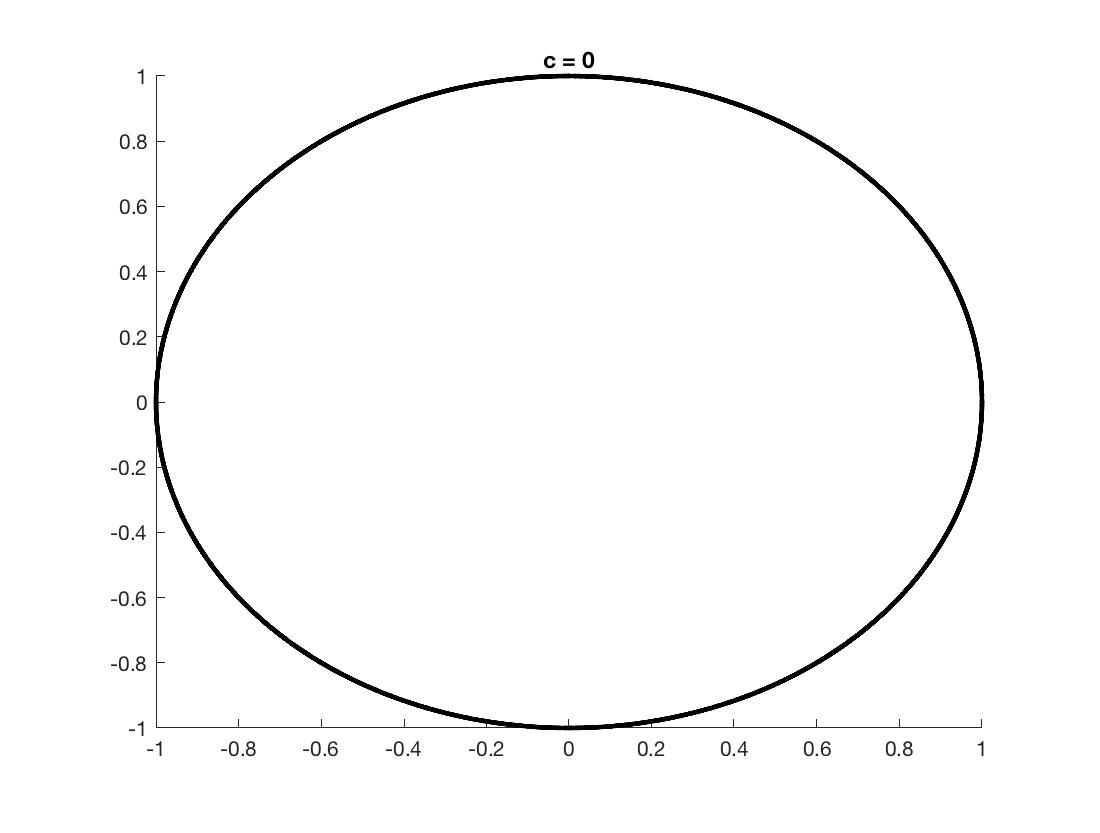
\includegraphics[width=\textwidth]{part3func1.eps}
    \caption{$c = 0$}
  \end{minipage}
  \hfill
  \begin{minipage}[b]{0.45\textwidth}
    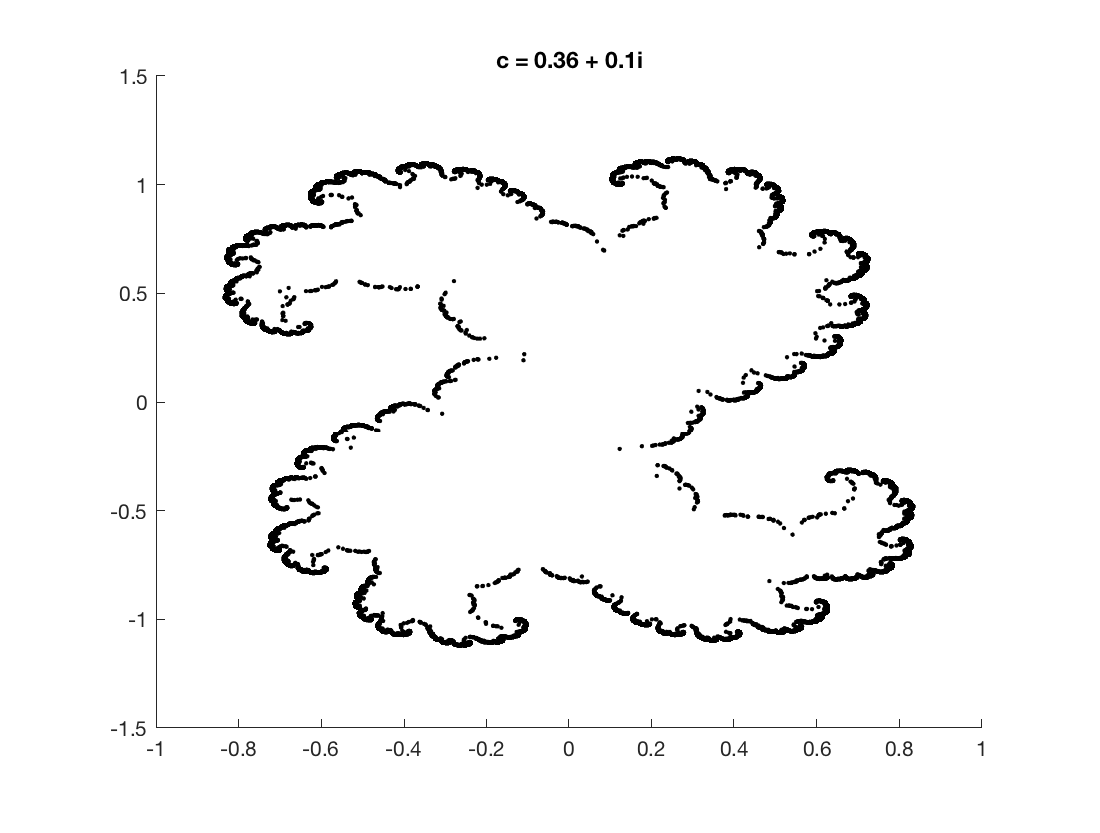
\includegraphics[width=\textwidth]{part3func2.eps}
    \caption{$c = 0.36 +  0.1i$}
  \end{minipage}
   \end{figure}
   
   \begin{figure}[H]
  \centering
  \begin{minipage}[b]{0.45\textwidth}
    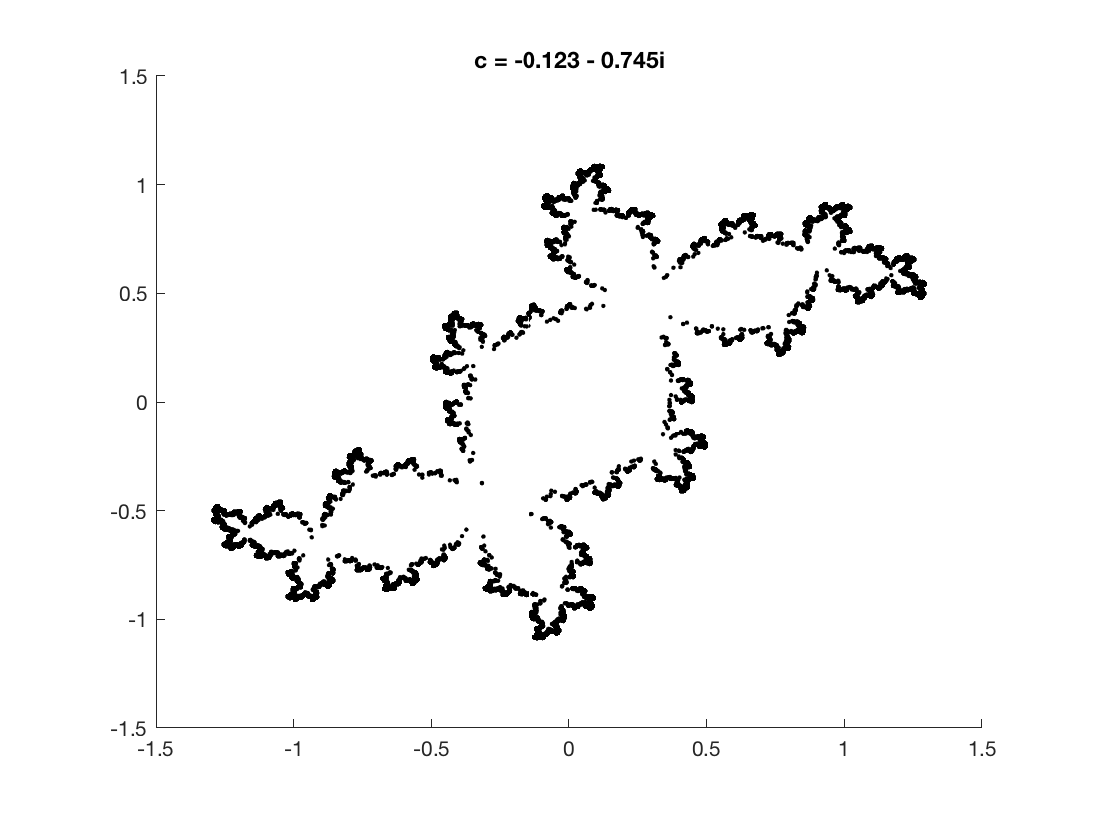
\includegraphics[width=\textwidth]{part3func3.eps}
    \caption{$c = -0.123 - 0.745i$}
  \end{minipage}
  \hfill
  \begin{minipage}[b]{0.45\textwidth}
    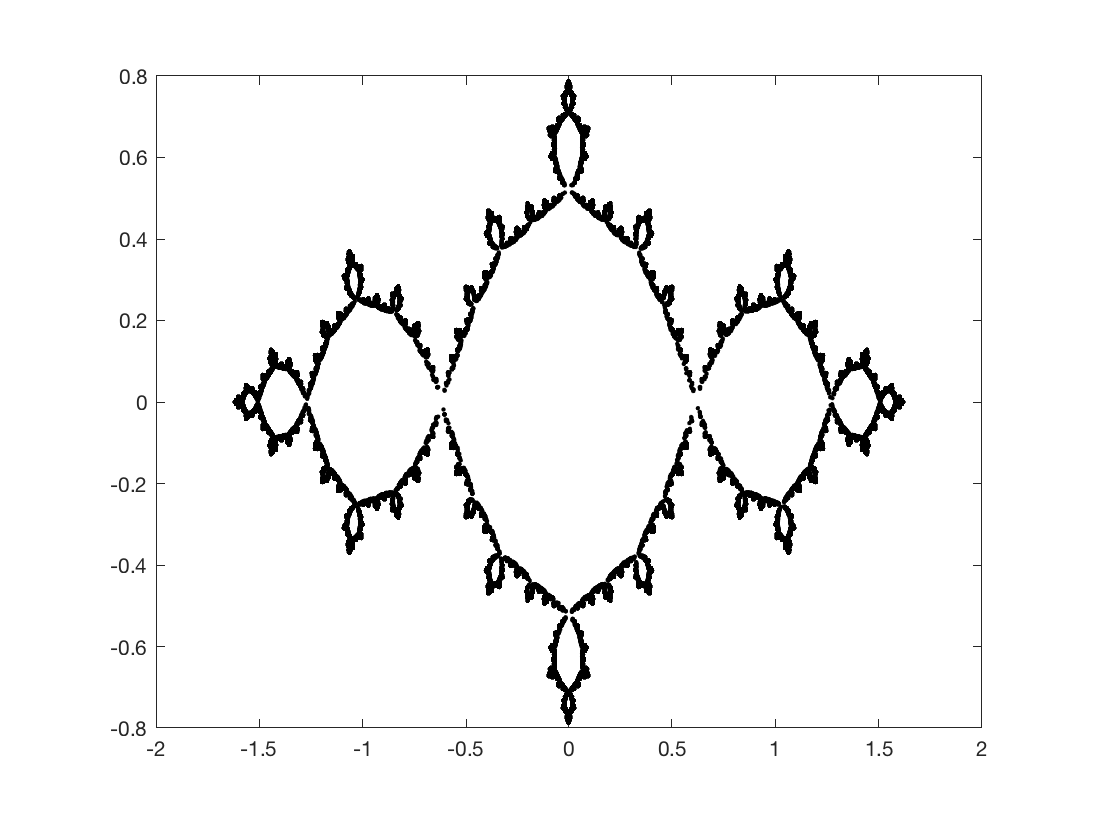
\includegraphics[width=\textwidth]{part3func4.eps}
    \caption{$c = -1i$}
  \end{minipage}
   \end{figure}
   
\section{Computing the Fractal Dimension}
Fractal dimension is a way of quantifying the level of self-similarity of a pattern. It is computed as the ratio of the number of self-similar copies to the measuring scale, in other words, it measures the complexity of a pattern. The more complex the pattern is, the larger its fractal dimension would be. Suppose we have a copy of fractal with a certain size, then we increase its size with magnitude $1/r$. Denote the number of self-similar copies of the original size to be $N$, then the dimension of this fractal is defined to be $$D = \frac{log(N)}{log(1/r)}$$
Consider a line segment, after double its length, the new line segment has two copies of the original one and thus has fractal dimension = 1.  If we double the edge length of a filled square, the new square is 4 times the original area containing 4 copies of the original filled square, thus has fractal dimension = 2.  Similarly, if we double the edge of a cube, the resulting structure will contain 8 copies of the original one, and thus has fractal dimension = 3. 
 \begin{figure}[H]
  \centering
  \begin{minipage}[b]{0.45\textwidth}
    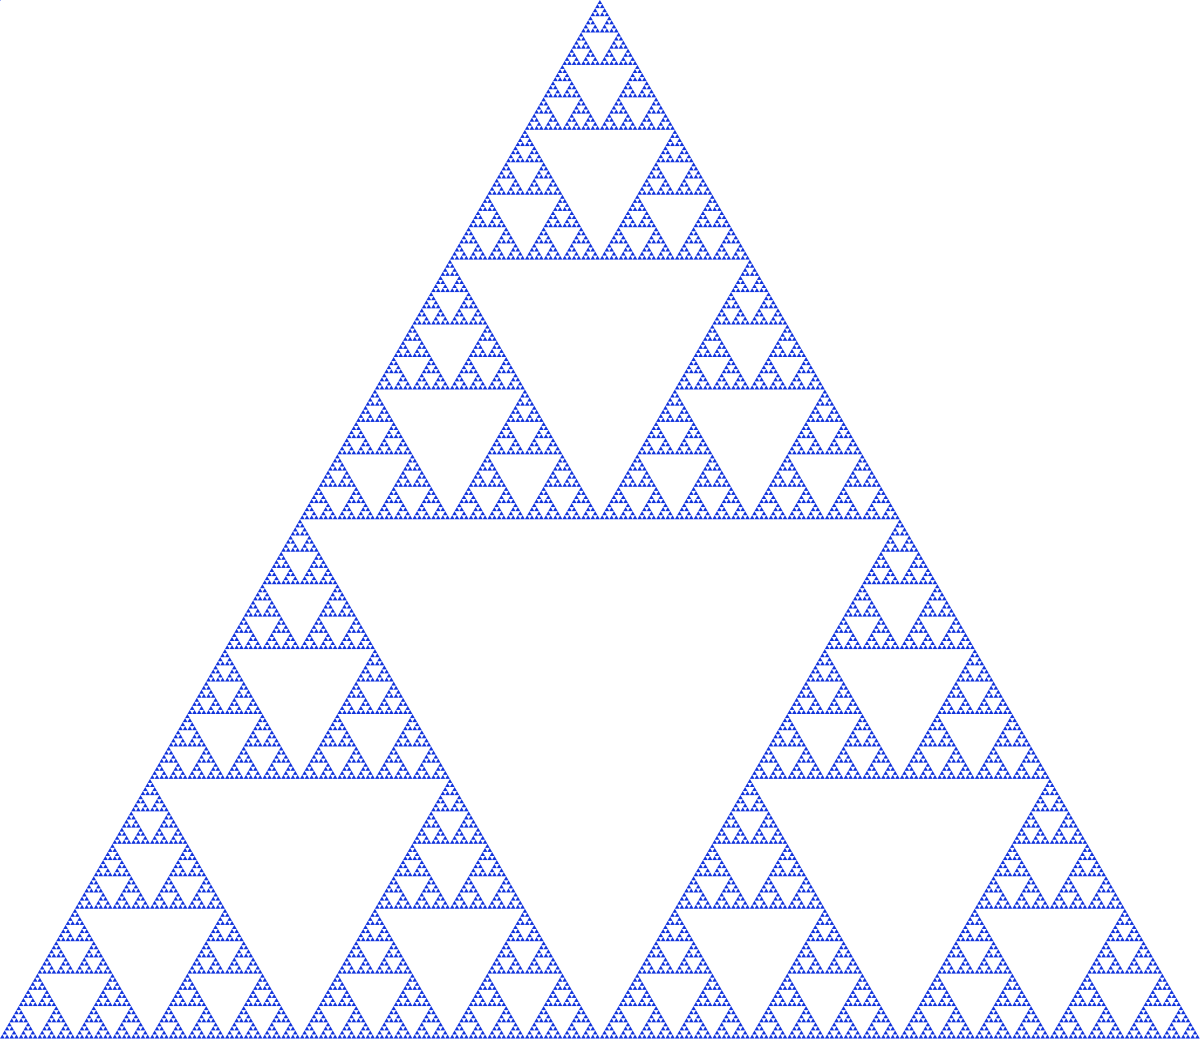
\includegraphics[width=\textwidth]{triag.png}
    \caption{sierpinski triangle (wikipedia)}
  \end{minipage}
  \hfill
  \begin{minipage}[b]{0.45\textwidth}
    \includegraphics[width=\textwidth]{snow.png}
    \caption{snow flaks: MrReid.org}
  \end{minipage}
   \end{figure}
The above examples all have integer fractal dimension, but fractal dimension can also be fractional. Consider the self similar triangle, each triangle is divided into four small triangles, and three of them are divided again. Accordingly, each small triangle is similar to the bigger one, which has half the magnitude. Besides, a big triangle has three such small triangles of half the magnitude. Thus the fractal dimension of sierpinski triangle: $$D = \frac{\log3}{\log2}.$$
Again, consider a snow flake, which is generated by iteratively adding triangles on the boundary. Each time, a single big edge of length $1$ is turned into four small edges of length $1/3$.  Magnifying the fractal by three times will generate 4 self similar copies, and thus the fractal dimension is $$D = \frac{\log(4)}{\log(3)}.$$

Yet, it is not the case that all the fractal dimensions can be calculated analytically. Thus, some methods can be used to approximate this value. One method is called box counting method. Basically, the method approximate the fractal dimension by measuring how the numbers boxes  required to cover the set changes as the box size gets finer. The dimension is approximated by the slope of log-log plot.

\textbf{Matlab Code -- Box Counting}:
\begin{lstlisting}
function D = box_count( IMG )
    %dim of image matrix
    %if the image is a curve with white background,
    %need to convert it: IMG = ~im2bw(IMG) then apply the algorithm
    dim = max(size(IMG));
    %in order to divide by half, want the size be 2^n
    dim = 2^ceil(log2(dim));
    %padding the matrix to square
    rowPad = dim - size(IMG, 1);
    colPad = dim - size(IMG, 2);
    IMG = padarray(IMG, [rowPad, colPad],0, 'both');
    imshow(IMG);
    boxCounts = zeros(1, ceil(log2(dim)));
    invr = zeros(1, ceil(log2(dim)));
    %intially, just one box
    num_boxes = 1;
    expo = 0;
    %while box is larger than 1x1, dim is box length
    while dim >= 1
        N(expo+1) = 0; %initialize count
        for box_row = 1:num_boxes
            for box_col = 1:num_boxes
                row_start = (box_row - 1) * dim + 1;
                row_end = box_row * dim;
                col_start = (box_col - 1) * dim + 1;
                col_end = box_col * dim;
                %i,e, 1~256,257~512,513~768, 769~1024
                
                contain_pixel = false;
                for row = row_start:row_end
                    for col = col_start:col_end
                        if IMG(row, col)
                            N(expo+1) = N(expo+1) + 1;
                            contain_pixel = true; % Break from nested loop.
                        end
                        %break inner
                        if contain_pixel
                            break; % Break from nested loop.
                        end
                    end %end inner inbox col loop
                    %break outer
                    if contain_pixel
                        break; % Break from nested loop.
                    end                   
                end %end outer inbox row loop
            end %end inner counting row of boxes loop
        end %end outer counting row of boxes loop
        
        % 2^expo = magnitude
        expo = expo + 1;
        invr(expo) = 1 / dim;
        
        num_boxes = num_boxes * 2;
        dim = dim / 2;
    end
    plot(log(invr),log(N));
    D = polyfit(log(invr), log(N), 1);
    D = D(1); %get the slope
end
\end{lstlisting}

\textbf{Matlab Code -- Differential Box Counting}:
\begin{lstlisting}
function D = dbc( IMG )
    %dim of image matrix
    dim = max(size(IMG));
    mymax = dim;
    %in order to divide by half, want the size be 2^n
    dim = 2^ceil(log2(dim));
    %padding the matrix to square
    rowPad = dim - size(IMG, 1);
    colPad = dim - size(IMG, 2);
    IMG = padarray(IMG, [rowPad, colPad],0, 'both');
    N = zeros(1, ceil(log2(dim)));
    G = zeros(1, ceil(log2(dim))+1);
    L = zeros(1, ceil(log2(dim))+1);
    K = zeros(1, ceil(log2(dim))+1);
    invr = zeros(1, ceil(log2(dim)));
    %intially, just one box
    num_boxes = 1;
    expo = 0;
    %while box is larger than 1x1, dim is box length
    L(expo+1) = 0;
    K(expo+1) = 0;
    while dim >= 1
        G(expo+1) = 0;
        N(expo+1) = 0; %initialize count
        for box_row = 1:num_boxes
            for box_col = 1:num_boxes
                row_start = (box_row - 1) * dim + 1;
                row_end = box_row * dim;
                col_start = (box_col - 1) * dim + 1;
                col_end = box_col * dim;
                %i,e, 1~256,257~512,513~768, 769~1024
                contain_pixel = false;
                %every box got 1, if max gray exists plus 1, if min
                %exists minus 1
                if(dim <= 128)
                N(expo+1) = N(expo+1) + 1;
                end
                
                for row = row_start:row_end
                    for col = col_start:col_end
                        if(dim <= 128)
                            if IMG(row, col) > 240%only consider the boxes with pixels
                                N(expo+1) = N(expo+1) + 1;
                                contain_pixel = true;
                            end
                            if IMG(row, col) < 8%only consider the boxes with pixels
                                N(expo+1) = N(expo+1) - 1;
                                contain_pixel = true; % Break from nested loop.
                            end
                        end
                        if(dim > 128)
                            if IMG(row, col)%only consider the boxes with pixels
                                N(expo+1) = N(expo+1) + 1;
                                contain_pixel = true;
                            end
                        end
                        %break inner
                        if contain_pixel
                            break; % Break from nested loop.
                        end
                    end %end inner inbox col loop
                    %break outer
                    if contain_pixel
                        break; % Break from nested loop.
                    end                   
                end %end outer inbox row loop
                
            end %end inner counting row of boxes loop
        end %end outer counting row of boxes loop

        expo = expo + 1;
        G(expo) = L(expo) - K(expo) + 1;     
        invr(expo) = mymax/dim;    
        num_boxes = num_boxes * 2;
        dim = dim / 2;
    end
     vpa([1./invr',N'])
    plot(log(invr),log(N));
    D = polyfit(log(invr), log(N),1);
    D = D(1); %get the slope
end
\end{lstlisting}

Using the unit circle generated in part1, and apply box counting method, we got dimension $\approx 1.2$, which should analytically be exactly 1. The error is still acceptable. Howeverm we cannot apply dbc method on such a curve, because it doesn have gray level. Then we used box counting method to approximate the dimention of koch snowflake and get $D \approx 1.375$. Its analytical dimension should be $log(4)/log(3) \approx 1.262$. We still want to say it is acceptable. Box counting method is not so accurate to approximate the dimension of a smooth curve like a unit circle.
\begin{figure}[H]
  \centering
  \begin{minipage}[b]{0.45\textwidth}
    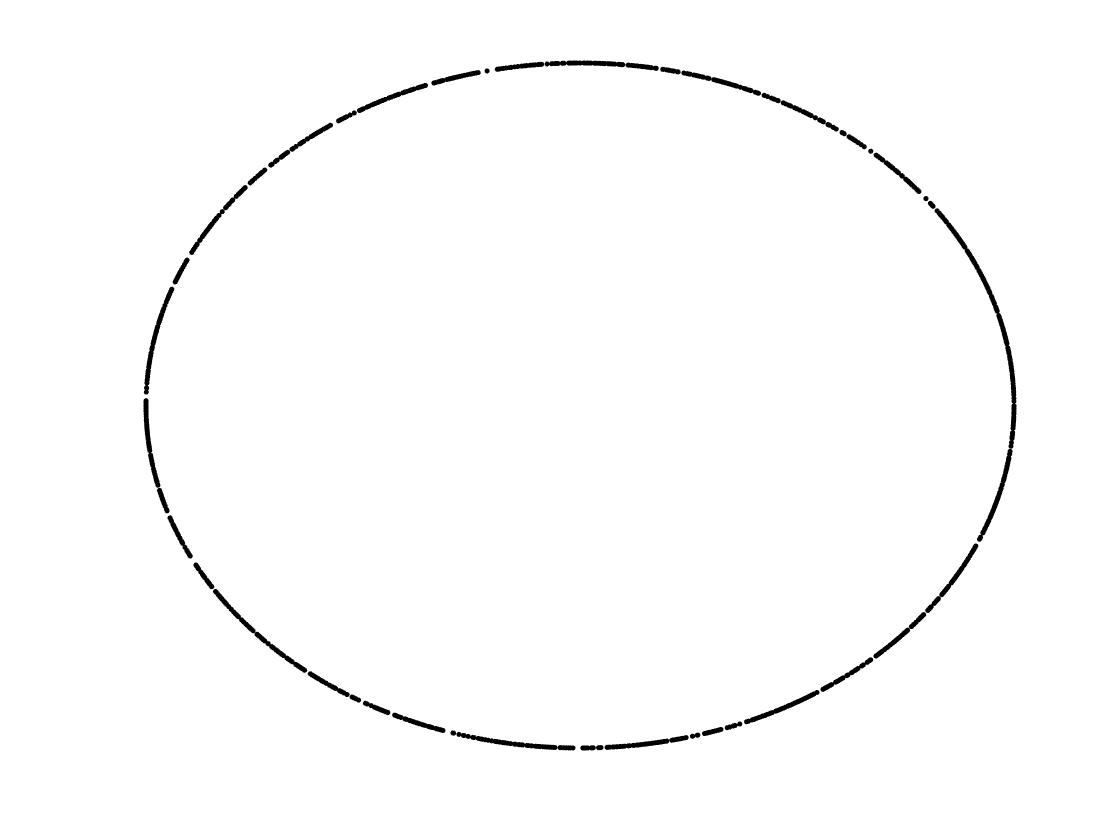
\includegraphics[width=\textwidth]{z2.jpg}
    \caption{unit circle generate by part1 (without axis for box counting}
  \end{minipage}
  \hfill
  \begin{minipage}[b]{0.5\textwidth}
    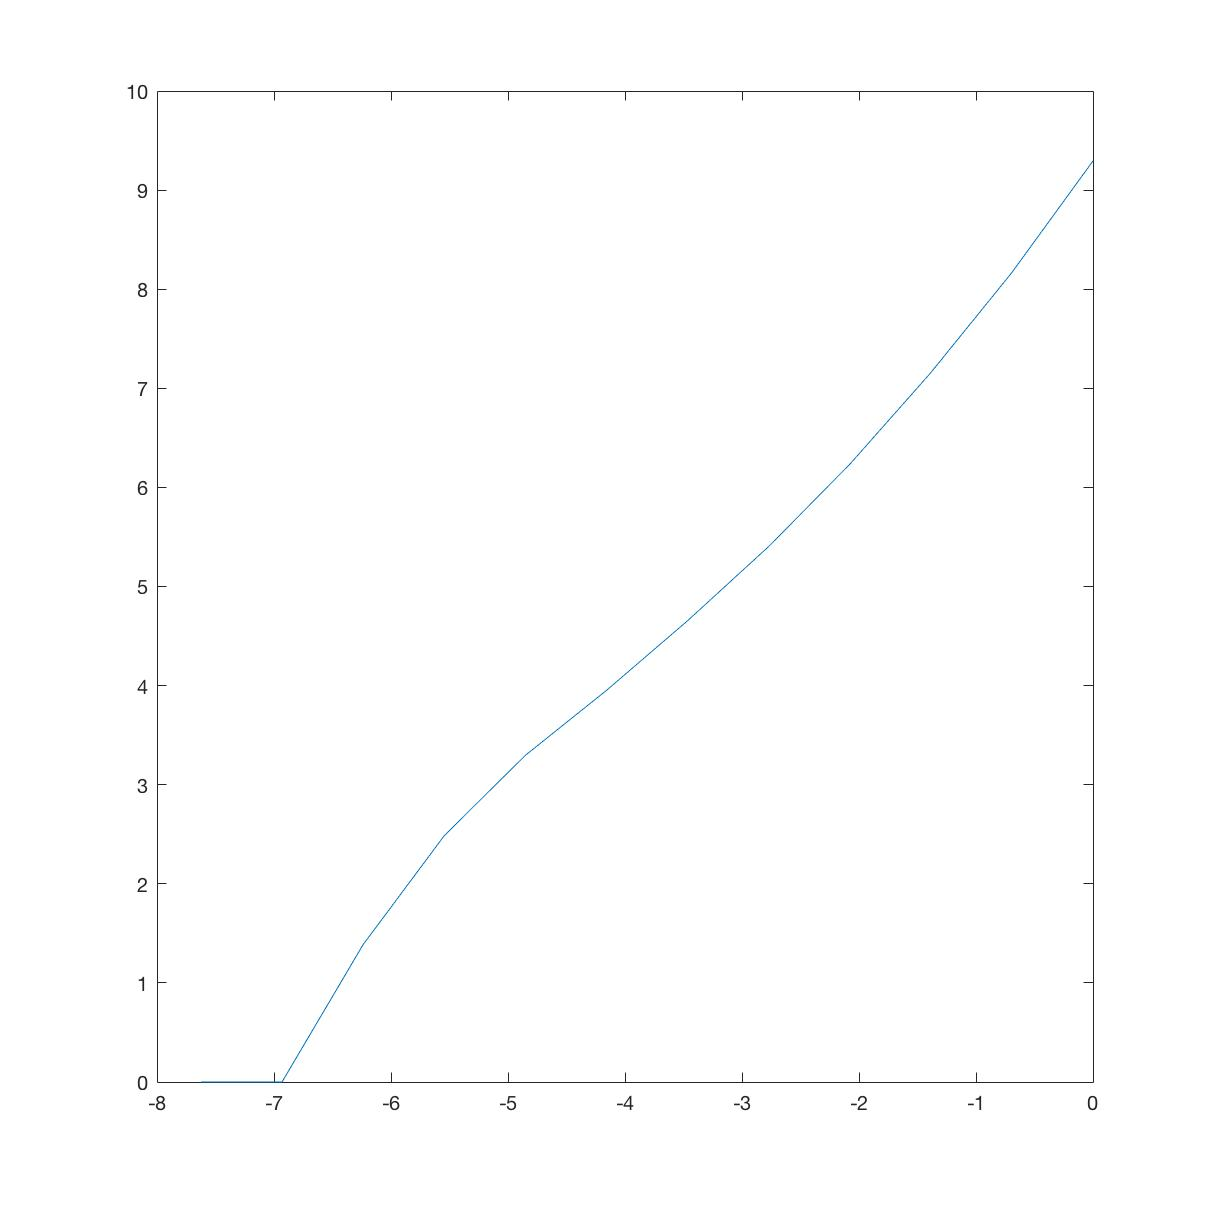
\includegraphics[width=\textwidth]{z2dim.jpg}
    \caption{polyfit for fractal dimension of unit circle}
  \end{minipage}
   \end{figure}
\section{Connectivity of the Julia Set}
A Julia set is connected if its orbit(0) is bounded. \\
To compute orbit(0), just apply the iteration method with $z_0 = 0$ and store the sequence $(z_i)$.\\
Assume divergence occurs when $|z| > 100$; if the orbit does not diverge after 500 iterations, consider it as bounded, which implies the corresponding Julia set is connected.\\
\textbf{MATLAB Code:}
\begin{lstlisting}
function [vec, connected] = orbit(x,y)
%vec: the orbit of 0 for phi(x) = x^2 + c, where c =x + iy
%connected : 0 if not connected, 1 if connected
z = x + 1i*y;
count = 1; %counter of number of iterations
connected = 0;

while abs(z) < 100
   vec(count) = z;%store the current z_n 
   count = count+1;
   z = z^2 + x + 1i *y; %z_{n=1} = z_n ^2 + c
   if (count > 500) %after 500 iterations, still not diverge
       connected = 1; %the julia set is connected
       break;
   end
end
end
\end{lstlisting}

\section{Coloring}
The code below uses nested for loops to check points diverge or not. If it diverge, then it shows really bright color.
\textbf{Matlab Code -- Coloring}:
\begin{lstlisting}
function [] = color( phi)
%phi is function handler,i.e., phi = @(z) z^3+1
%returns the RGB triplet for divergent orbit
%if convergent, black
count = 1;

M = zeros(200);
for x = 1:400
    for y = 1:400
           z = 0.01*(x-1)-2 - 0.01i*(y-1) + 2i;
           count = 1;
           bounded = false;
        while abs(z) < 100 & count < 1500
           count = count+1;
           % the fixed point function can be modified here
           z = phi(z);
           if(abs(z) >= 100)
            M(x,y) = 10*count;
           end
        end

    end
end
figure
image([-2 2],[-2 2],M')
end
\end{lstlisting}
Note: Although the points on imaginary axis are from bottom = 2 to top = -2, it is actually the reverse. The real and imaginary axis are actually in regular directions, but I cannot make it show correctly.
\begin{figure}[H]
  \centering
  \begin{minipage}[b]{0.49\textwidth}
    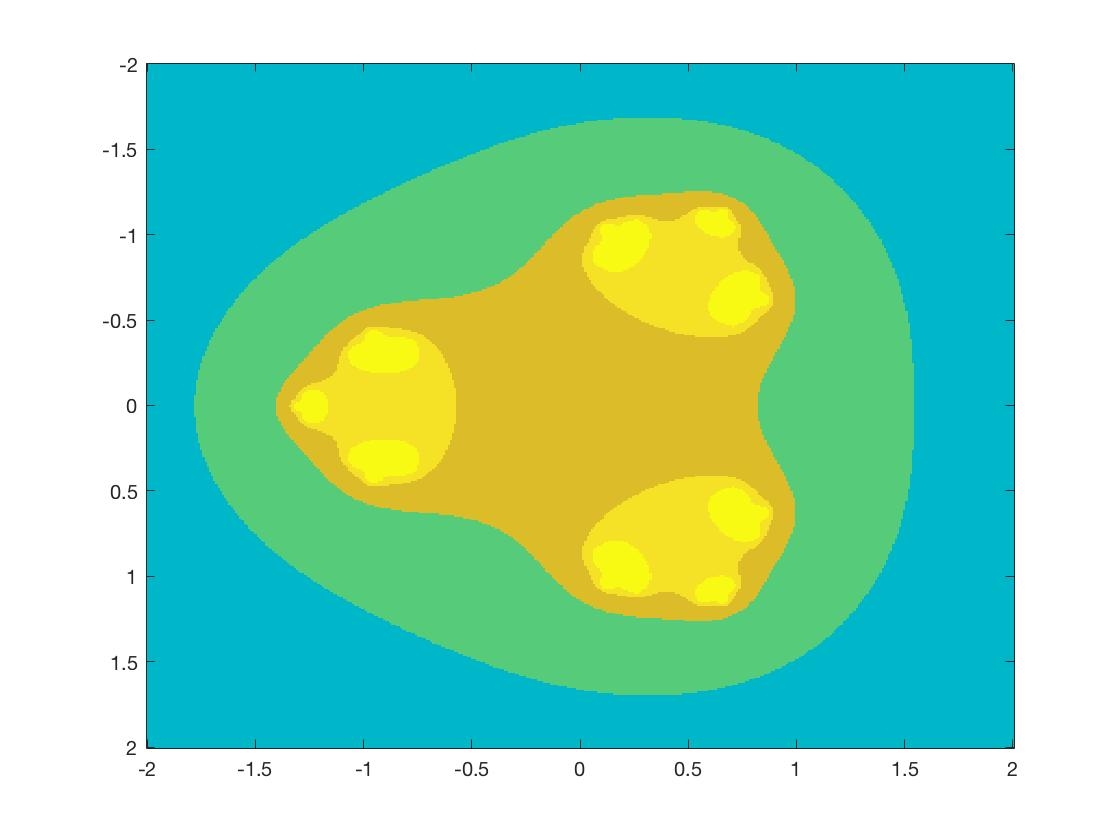
\includegraphics[width=\textwidth]{z3+1.jpg}
    \caption{$z^3+1$}
  \end{minipage}
  \hfill
  \begin{minipage}[b]{0.5\textwidth}
    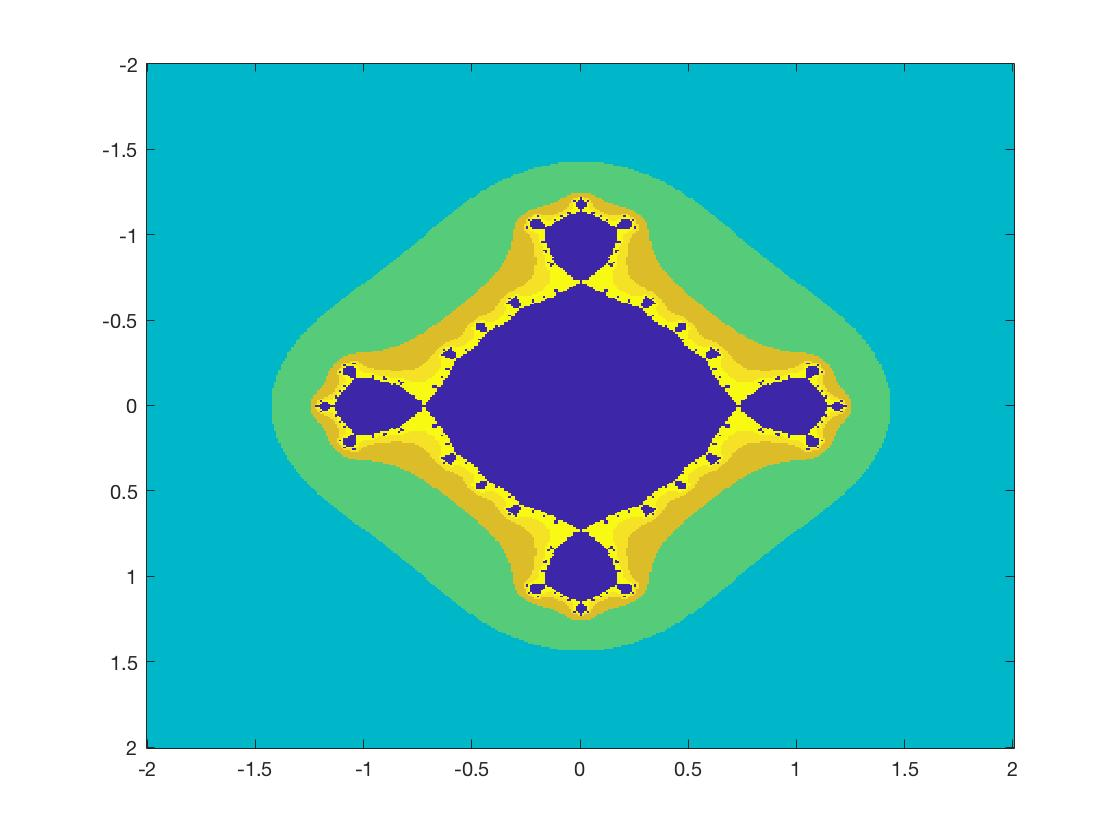
\includegraphics[width=\textwidth]{z4-1.jpg}
    \caption{$z^4-1$}
  \end{minipage}
  \end{figure}
  \begin{figure}[H]
  \centering
    \begin{minipage}[b]{0.49\textwidth}
    \includegraphics[width=\textwidth]{z4-06+03i.jpg}
    \caption{$z^4-0.6+0.3i$}
  \end{minipage}
  \hfill
  \begin{minipage}[b]{0.5\textwidth}
    \includegraphics[width=\textwidth]{z2-06+03i.jpg}
    \caption{$z^2-0.6+0.3i$}
  \end{minipage}
   \end{figure}
\section{Newton's Iteration}
\textbf{Newton's Iteration Matlab Code with coloring implemented}
\begin{lstlisting}
%Solving z^3 - 1 = 0
f = @(z) z^3 -1;                    
fprime = @(z) 3*z^2;
phi = @(z) z - f(z)/fprime(z); %fixed point iteration
M = zeros(200);
flag = 0;
hold on
for x = 1:400
    for y = 1:400
           z = 0.01*(x-1)- 2 + 0.01i*(y-1) - 2i;
           count = 1;
           flag = 0;
        while abs(z) < 100 && count < 1500
           count = count+1;
           % the fixed point function can be modified here
           temp = phi(z);
           if(abs(temp - z) <= 10^-8)
               flag = flag + 1;
           end
           z = temp;
           if(flag >= 10)
               M(x,y) = ceil(0.7*count);
               break;
           end
           if(abs(z) >= 100)
            M(x,y) = 300;
            break
           end
        end
    end
end
figure
image([-2 2], [-2 2], M')
\end{lstlisting}
\begin{figure}[H]
    \centering
    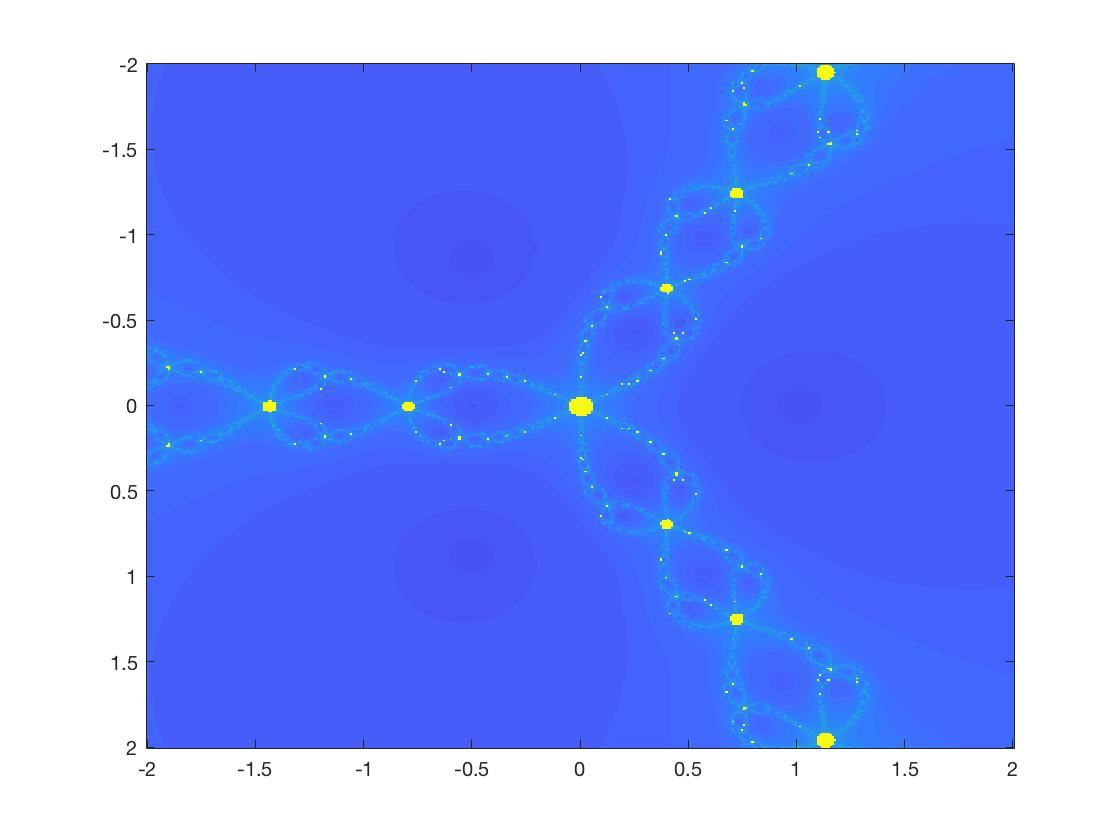
\includegraphics[width=0.9\textwidth]{z^3-1.jpg}
    \caption{newton: $z^3-1$}
\end{figure}
    As show by the figure, the roots locate at the darkest blue area, while points within the bright yellow area diverge really fast.

\section{Mandelbrot Set}
The Mandelbrot set is the set of points $c$ for which the Julia set is connected.\\
Therefore, to generate the Mandelbrot set, one can select of a set of $c$ values (here $c = x+iy$ is chosen in the range of $x \in [-2,1]$ and $y \in [-1.5,1.5]$). For any $c$, check whether the associated Julia set is connected using the function from part 5. If so, color the point $c$ as black; otherwise, the color of $c$ depends on the number of iterations it takes for the sequence to diverge ($|z| > 100$).\\
\textbf{MATLAB Code:}
\begin{lstlisting}
function [] = MandelbrotSet()
%generate the MandelBrot set
numColor = 20; %number of different colors
N = zeros(numColor,3);
for i = 1: numColor %generate the matrix for colormap with varying colors
    colorValue = i * (1/numColor);
    N(i,:) = [colorValue colorValue colorValue];
end

colormap(N); %create the colormap
inc = 0.005;
iteration = 3/inc + 1;%the range of x and y are both 3

M = 2*ones(iteration, iteration);

for i = 1:iteration
    x = -2 + (i-1) * inc; %x(real) from -2 to 1
    for j = 1:iteration
        y = -1.5 + (j-1) * inc; %y(imaginary) from -1.5 to 1.5
        [count, connected] = orbit(x,y); %computes the connectivity
        if(connected)%connected, set to black
            M(j,i) = 1;
        else %not connected, set to corresponding color
            M(j,i) = count;
            
        end
    end
    
end
    figure(1);
    image([-2, 1],[-1.5,1.5],M);
	set(gca,'XTick',[]) % Remove the ticks in the x axis!
	set(gca,'YTick',[]) % Remove the ticks in the y axis
	%set(gca,'Position',[0 0 1 1]) % Make the axes occupy the hole figure
	saveas(gcf,'mand','jpg');% generate png for dimension use
    
end

function [count, connected] = orbit(x,y)
%count: the number of iterations it takes to diverge
%connected : 0 if not connected, 1 if connected
z = x + 1i*y;
count = 1;
connected = 0; %counter for number of iterations
while abs(z) < 100 %assume divergence occurs when |z| > 100
   count = count + 1;
   z = z^2 + x + 1i *y; %z_{n+1} = z_n^2 + c
   if (count >= 500) %after 500 iterations, still not diverge
       connected = 1;
       break;
   end
end
end
\end{lstlisting}
 \begin{figure}[H]
  \centering
    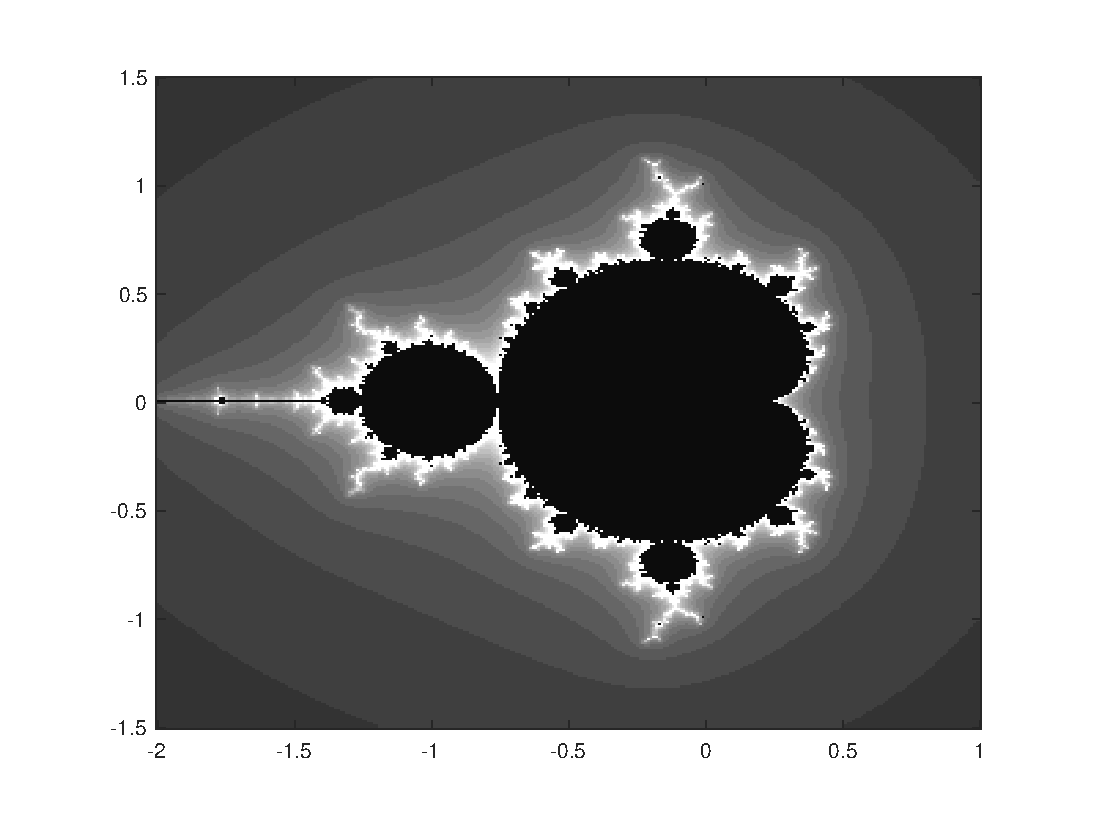
\includegraphics[scale=0.75]{Mandelbrot.eps}
    \caption{Mandelbrot Set}
   \end{figure}
   
   
   
\section{Work Distribution}
Xinke: part 3, part 5, part 8\\
Xuanchen: part 4, part 6, part 7
\end{document}
